\documentclass[12pt,oneside,a4paper]{article}
\usepackage[utf8]{inputenc}
\usepackage[T1]{fontenc}
\usepackage[hungarian]{babel}
\usepackage{graphicx}
\usepackage{amsmath}
\usepackage{glossaries}
\usepackage{hyperref}
\usepackage{fancyhdr}
\usepackage{enumitem}
\usepackage[headheight=15mm, footskip=10mm]{geometry}
\usepackage{makeidx}
\usepackage{url}
\usepackage{times}
\usepackage[printonlyused,withpage]{acronym}
\usepackage{tikz}
\usepackage{tabularx}
\usepackage{pdfpages}
\usepackage{wrapfig}

\newcommand{\newsection}[1]{\clearpage\section{#1}}\label{makro}
\newcommand*{\titletext}{Yolov8-as szegmentációs háló és annak magyarázhatósága EigenCAM típusú modellfüggetlen magyarázó rendszerrel}

\usepackage{amsthm}

\theoremstyle{remark}
\newtheorem*{remarkth}{Válasz: \newline}
\newenvironment{remark}{\begin{remarkth}}{\end{remarkth}}
\newcommand{\oldh}{\("old\)}\label{makro2}
\newcommand{\newh}{\("new\)}
\newenvironment{kerdes}{
    \medskip%
    \par\noindent\ignorespaces%
    \textsc{\textbf{Kérdés: }}%
    \medskip
    \textsf%
    %
        }{%
        \medskip
}

\makeindex
\makeglossaries

\newglossaryentry{Yolo}
{
    name=You Only Look Once,
    short=YOLO,
    description={You Only Look Once, egy gyors és hatékony objektumdetektáló neurális hálózat}
}
\newglossaryentry{Yolov8}{
short=YOLOv8,
name=You Only Look Once version 8,
description={A YOLOv8 egy hatékony és népszerű szemantikus szegmentációs hálózatcsalád legújjabb példánya}
}

\newglossaryentry{github}
{
    name=GitHub,
    description={Egy webes szolgáltatás, amely Git verziókövető rendszert használó szoftverfejlesztési projektek tárolására és verziókövetésére szolgál}
}
\newglossaryentry{EigenCAM}{
name=Eigen Class Activation Mapping,
short=EigenCAM,
description={Egy modellfüggetlen magyarázó rendszer, amely képes vizualizálni, hogy a mély tanuló hálózatok mely részei járultak hozzá a döntéshozatalhoz}
}
\newglossaryentry{Yolov5}{
short=YOLOv5,
name=You Only Look Once version 5,
description={A YOLOv5 egy hatékony és népszerű objektumdetektáló neurális hálózat}
}
\newglossaryentry{Inference}{
name=Inference,
description={Az inferencia a gépi tanulásban a modell által megtanult minták alkalmazását jelenti új adatokon}
}
\newglossaryentry{epoch}{
name=epoch,
description={Az Epochok száma adja meg hányszor megy végig a tanulás során a hűló a teljes adathalmazon}
}
\title{\titletext}
\author{Nyilas Péter}
\date{\today}



\pagestyle{fancy}
\fancyhf{}

% Header
\fancyhead[L]{
    \includegraphics[width=4cm]{BMElogo}
}
\fancyhead[R]{
    \includegraphics[width=1cm]{MITlogo}
}
\renewcommand{\footrulewidth}{0.4pt}
\pagestyle{fancy}

% Footer
\fancyfoot[L]{
    \footnotesize
    Budapest Műszaki és Gazdaságtudományi Egyetem \\
    Villamosmérnöki és Informatikai Kar \\
    Méréstechnikai és Információs Rendszerek Tanszék \\
    \url{www.mit.bme.hu}
}
\fancyfoot[R]{
    \raisebox{-0.9\height}{\includegraphics[width=0.9cm]{viklogo}}
    \thepage
}

\makeglossary

\begin{document}

\maketitle
\newpage
\tableofcontents\label{ossz:tartalomjegyzek}
\newpage
\newsection{Bevezetés}\label{sec:bevezetes}
\pagestyle{fancy}
% Bevezetés a YOLOv8 szegmnetációs hálózathoz és az interpretálhatóság fontosságához.
    % A magyarázhatóság szerepe a mély tanuló modellek értelmezhetőségében és elfogadhatóságában.
    A tavalyi témalaboratóriumi dolgozatomban is foglalkoztam közlekedési objektumok detektálásával,
    a gépi látás (\ac{CV}) témakörében, mindezt Yolo architektúrájú neurális hálóval akkor a
\glsentryshort{Yolov5}-el, ebben a dolgozatban megfogalmaztam terveket az eredmények javításában, ezek mentén végeztem
a következőkben leírt munkámat:
\begin{enumerate}[label=\alph*., start=1]\label{enum:tervek}
    \item Újabb/nagyobb háló alkalmazása
    \item Áttérni a szemantikus szegmentációra bounding boxról
    \item Új (hardveres) erőforrással és jobb szoftveres kiszolgálás
\end{enumerate}
Ezekhez még hozzáadódott az, hogy vizsgáljam mellé, hogy
\begin{enumerate}[label=\alph*., start=3]
    \item a háló döntéseit hogyan lehetne magyarázni, hogy azokat \textit{"debugolhatóvá"} érthetőbbé tegyem.
\end{enumerate}


    Szakmai gyakorolatomban is képfeldolgozó neurális hálókkal foglalkoztam és itt megtapasztalhattam hogy az ilyen
    hálózatok azonban gyakran fekete    dobozként működnek, ami komplikálttá teszi azok megértését az
    emberi felhasználók számára, akik meg szeretnék érteni    a működésüket hogy biztonságosabbnak tudhassuk ezeket,
    és megértésükkel későbbi hibákat javíthassunk.Az interpretálhatóság, vagyis a modell döntéseinek megértés
    és magyarázata, ezért kulcsfontosságú az ilyen modellek elfogadhatóságában és alkalmazhatóságában.

    A YOLOv8 (\gls{Yolov8}) egy népszerű és hatékony ilyen neurális háló,
    ennek is a szemantikus szegmentációs változatát használom (Yolov8m\_seg), amely számos alkalmazásban használatos,
    például objektumfelismerésben és objektum-klasszifikációban.
    Annak érdekében, hogy jobban megértsük és magyarázni
    tudjuk ennek hozott döntéseit, olyan magyarázó rendszerekre van szükségünk, amelyek képes betekintést nyerni a
    modell működésébe.

    Egy ilyen eszköz az \glsentryshort{EigenCAM} (\gls{EigenCAM}) egy ilyen modellfüggetlen magyarázó rendszer,
    amely képes vizualizálni, hogy a mély tanuló hálózatok mely részei járultak hozzá a döntéshozatalhoz.
    Ehhez pedig
    az aktivációs függvények értékeit kiemeli a hálóból és a képre vetíti amire ezt futtatjuk, majd ezeket kombinálja
    egy képpé megmutatva azt hogy melyik részei a képnek milyen fontosak a döntések meghozásában.

\newsection{Mély tanulás és interpretálhatóság}\label{sec:mely-tanulas-es-interpretalhatosag}
% Áttekintés a mély tanulás elméletéről.
    % Miért fontos az interpretálhatóság a mély tanuló modellekben?
    % Különböző magyarázó módszerek áttekintése.
A Mesterséges intelligenciát használó megoldásokat azért használjuk gyakran hogy rugalmasabb megoldást adjon akár
nehezen algoritmizálható problémáinkra.
Azonban ezek a modellek gyakran rendkívül bonyolultak és nehezen
 értelmezhetőek az emberi számára.
 Ezért elengedhetetlen az interpretálhatóság, vagyis annak képessége, hogy a modellek
döntéseit érthető és ésszerű módon magyarázza meg.

 A mély tanulási modellek interpretálhatósága fontos szempont minden alkalmazásban.
 Például a klinikai diagnosztikában
fontos tudni,
 automatikus döntés miért született, hogy az orvosok megbízhatóan megérthessék és elfogadhassák az eredményt.
 Forgalmi
szituációban miből vett észre vagy nem vett észre objektumokat

    Különböző magyarázó módszerek léteznek a mély tanulási modellek interpretálhatóságának növelésére.
    Ezek közé
tartoznak olyan módszerek is amely egy egyszerűbb
neurális hálót tanít be hasonló dolgokra mint amire a hálónkat tanítjuk ,ezek a modellfüggő magyarázó módszerek.
Léteznek azomban modellfüggetlen megoldások például az attribúciós módszerek
, a visszafejtési technikák és a modellek folyamatos monitorozására alkalmas szoftverek.
Az egyik ilyen monitorozó módszer az \glsentryshort{EigenCAM} (\ref{sec:eigencam:-modellfuggetlen-magyarazo})\label{sechiv}.


\begin{kerdes}
    Miért is ilyen fontos a modell interpretálhatósága és a magyarázhatósága?
\end{kerdes}
\begin{remark}
    Különösen fontos a jogi szabályozásban egy ilyen modell használatakor, hogy a döntések átláthatóak és
    érthetőek legyenek.
    Például az Európai Unió által 2016-ban életbe léptetett Általános Adatvédelmi Rendelet (GDPR) előírja, hogy az
    automatizált döntéshozatalnak átláthatónak kell lennie, és az érintetteknek joguk van tudni, hogy egy algoritmus
    milyen döntéseket hoz róluk.
\end{remark}
\newsection{YOLOv8: Szemantikus szegmentációs háló és működése}\label{sec:yolov8:-szemantikus-szegmentacios-halo}
% Rövid áttekintés a YOLOv8 szegmentációs hálóról.
    % Funkcionális működésének magyarázata.
    % Teljesítmény és pontosság értékelése.
    A YOLOv8 (\cite{Yolov8})\label{irodalomhivatkozas} egy hatékony és népszerű szemantikus szegmentációs hálózatcsalád legújjabb példánya,
    amelyet számos számítógépes látás (\ac{CV})
    feladatban használnak.
    A \("You Only Look Once"\) (\glsentryshort{Yolo}) megközelítést alkalmazza,
amely gyors és pontos objektumdetektálást tesz lehetővé egyetlen neurális háló segítségével.

\begin{wrapfigure}{l}{0.2\textwidth}
  \centering
  \includegraphics[width=\linewidth]{Ultralytics}
  \caption{Ultralytics}
  \label{fig:Ultralytics}
\end{wrapfigure}
    A YOLOv8 működése során a bemeneti képet egyszerre veszi figyelembe, és az objektumok pozícióját
és osztályát egyetlen predikcióval határozza meg.
Ez a modell különösen alkalmas valós
idejű alkalmazásokhoz, mint például az önvezető járművek vagy a videoelemzés.

    A YOLOv8-nak kiváló teljesítménye és pontossága van, ami azt jelenti,
hogy gyorsan és pontosan k  wépes azonosítani az objektumokat a képeken és videókon.

Ennek a hálónak én a szegmentációs változatát használtam, amely mostanság egy eléggé új
irány a közlekedési objektumok detektálásában, eddig ugyanis inkább 2--3 dimenziós ún. \("\)bounding boxokat\("\)
azaz kereteket használtak az objektumok azonosítására, azonban a szegmentációs hálók képesek az objektumok
pontosabb azonosítására és lokalizálására, azaz az objektumok pontos körvonalainak meghatározására.
Ezáltal a szegmentációs hálók pontosabb és részletesebb információkat nyújtanak az objektumokról, mint a keretes
interpretáció.


\subsection{Szemantikus szegmentáció}\label{subsec:szemantikus-szegmentacio}

A szemantikus szegmentáció\index{szemantikus szegmentáció} egy olyan számítógépes látás feladat, amelyben a cél az objektumokat tartalmazó kép egyes
részeinek (például pixeljeinek) címkézése az objektumokhoz tartozó osztályok szerint.
Más szavakkal, minden képpontot
hozzá kell rendelni egy osztályhoz vagy kategóriához, például autó, biciklis, gyalogos stb.
Ezáltal a szemantikus szegmentáció
lehetővé teszi a \glsentryshort{Computer Vision} rendszereknek, hogy pontosan azonosítsák és lokalizálják az
objektumokat egy adott képen.
Fontos megjegyezni hogy egy nagy különbség a szemantikus és az egyed szegmentáció között,
hogy az egyed szegmentációban minden objektumot külön kell azonosítani, míg a szemantikus szegmentációban csak az
objektumok osztályait kell meghatározni.

Tehát a szemantikus szegmentációt leírhatjuk úgy, ha egy képet jelölünk \(I\) -vel, akkor a szemantikus
szegmentáció pedig egy olyan függvény,\(F: I \rightarrow L\), ahol \(L\) a lehetséges osztályok halmaza, és \(F\) minden
képpontot hozzárendel egy osztályhoz.

A szemantikus szegmentáció kiemelt fontosságú az önvezető autók, a
,videoelemzés, a térképek építése és sok más
alkalmazásban, ahol pontos és részletes objektumfelismerésre van szükség.


\subsection{Adathalmazok és kísérletek}\label{subsec:adathalmazok-es-kiserletek}
    % Bemutatás és elemzés a használt adathalmazokról.
    % Kísérletek és eredmények az EigenCAM alkalmazásával a YOLOv8-ra.
\pagestyle{fancy}
    Adathalmazként (Datasetnek) , témalaboratóriumhoz hasonlóan a CityScapes\index{CityScapes}
    (\url{https://www.cityscapes-dataset.com}) adathalmazt, annak is a finoman annotált (Fine Annotated),\aref{fig:CityScapes-Examples}\label{kephivatkozas}.képen bemutatott,
adathalmazát használtam ami osztályszegmentációs maszkokat biztosít a képeihez ami ~ 5000 kép, közlekedési szituációkban, elég nagy
varianciával rendelkezik ahhoz hogy egy robosztus szegmentációs hálót tudjunk tanítani közlekedési objektumok
detektálására.
A Magyarázat a ~\pageref{subsec:magyarazat}\label{pageref}. oldalon található.


    \begin{figure}[h]
       \centering
        \noindent\includegraphics[width=1\linewidth]{cityscapes}
        \caption{CityScapes Examples}
        \label{fig:CityScapes-Examples}
    \end{figure}
    Ezeket az adatokat fogjuk a későbbiekben használni arra hogy megpróbáljuk megérteni a hálónkat az aktvivációi
    alapján.
    Ezeket a teszteket a Bonn-i teszt halmazon végeztem.

\newsection{EigenCAM: Modellfüggetlen magyarázó}\label{sec:eigencam:-modellfuggetlen-magyarazo}
% Mi az EigenCAM és hogyan működik?
    % Az EigenCAM előnyei és korlátai.
    % Az EigenCAM alkalmazása különböző típusú modellekre.
     Az \glsentryshort{EigenCAM}index{EigenCAM} (Eigen Class Activation Mapping) egy modellfüggetlen magyarázó rendszer, amelyet a mély tanulási
     modellek interpretálhatóságának növelésére fejlesztettek ki.
     Az \glsentryshort{EigenCAM} célja, hogy vizualizálja és magyarázza meg a modellek döntéseit a bemeneti adatok alapján,
     osztálydiszkrimináció nélkül.

    Az \glsentryshort{EigenCAM} működése során az algoritmus az egyes osztályokhoz tartozó aktivációs térképeket számolja ki,
     majd ezeket kombinálja az osztályok jellemzőinek és fontosságának megjelenítéséhez.
    Ez lehetővé teszi, hogy az emberi felhasználók megértsék, hogy a modell miért döntött úgy, ahogy.

    Az \glsentryshort{EigenCAM} előnyei közé tartozik a modellfüggetlenség és a viszonylag egyszerű megvalósítás.
     Azonban fontos tudni, hogy az \glsentryshort{EigenCAM} csak egy interpretálhatósági eszköz, és nem biztosít teljes képet
     a modell működéséről.
    \begin{remark}
        Az akticvációs függvények a modell layereinek kimeneti függvényei ahol \("x\) az input, \("W"\) a súlymátrix és \("b"\) a
    bias vektor.
        Az utolsó layerben egy lineáris aktivációs~\eqref{eq:RELU}\label{alignhivatkozas} függvényt használunk, míg az összes többi layerben egy
    szivárgó rektifált lineáris aktivációt~\eqref{eq:LRELU}\label{eqhivatkozas} használunk:
    \end{remark}
    \begin{equation}
        \text{ (LRELU):}
    \varphi(x) = \begin{cases}
      x, & \text{ha } x > 0 \\
      0.1x, & \text{különben}
    \end{cases}\label{eq:LRELU}
    \end{equation}\label{eq:activation_functions}


    \begin{align}
    \text{RELU:}
    \varphi(x)=\begin{cases}
      x, & \text{ha } x > 0 \\
      0, & \text{különben} \end{cases}\label{eq:RELU} \\
    \text{Sigmoid:}
    \varPhi(x) &= \frac{1}{1 + e^{-x}} \label{eq:Sigmoid}
    \end{align}



\newsection{Az EigenCAM alkalmazása a YOLOv8-ra}\label{sec:az-eigencam-alkalmazasa-a-yolov8-ra}
% Hogyan alkalmazható az EigenCAM a YOLOv8 szegmentációs hálóra?
    % Konkrét példák és esettanulmányok.
    Az \glsentryshort{EigenCAM}index{EigenCAM} alkalmazása a YOLOv8 szemantikus szegmentációs hálóra lehetővé teszi számunkra, hogy megértsük,
    hogy a modell miként dönt az objektumok azonosításáról és lokalizálásáról a képeken és videókon.

    A konkrét Működési folyamata \aref{fig:flowchart}\label{abrahiv} ábránlátható.
    A CityScapes adathalmazon tanítottuk a YOlov8m-seg hálót, majd az EigenCAM segítségével vizualizáltuk az aktivációkat,
    amelyek a háló a képek feldolgozása közben produkál (ezt az EigenCAM adja a hálónak egy olyan folyamaton keresztül
    amit \gls{Inference}-nek nevezünk), ezeket az EigenCAM kivezeti és rávetíti a bemenő képre (ezt a folyamatot lásd
    \aref{fig:flowchart} képen és\aref{Inference} pontban \label{listahiv} ), a különböző
    héjak aktivációit külön-külön.
    Amikor végez a kép előállításával azt HEATMAP formájában az output mappájába helyezi.

\begin{center}
    \resizebox{1\textwidth}{!}{%
        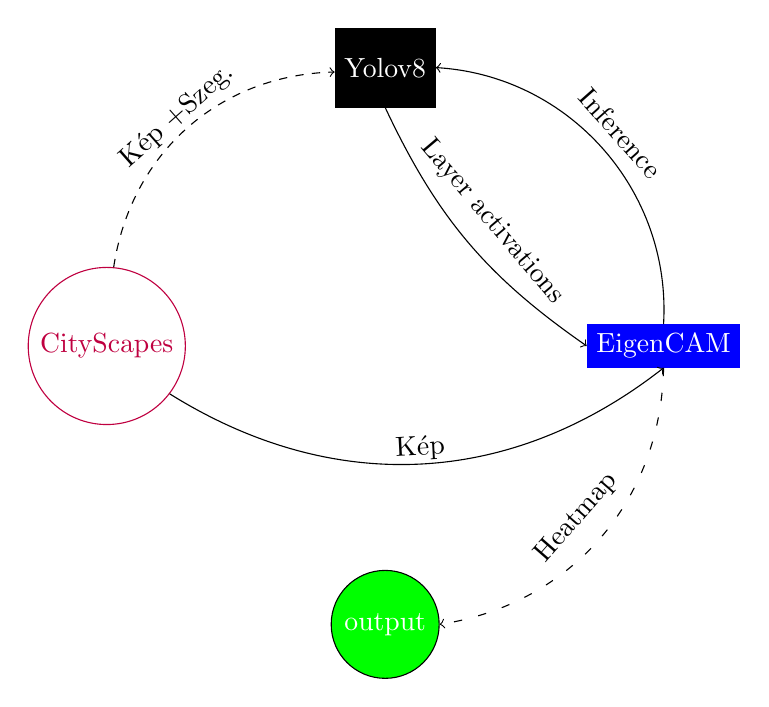
\begin{tikzpicture}
            \begin{scope} [node distance=5cm]
                \node[shape=circle, draw, color=purple] (CityScapes) {CityScapes};
                \node[shape=rectangle, draw, color=black, fill=black,
                    text=white, minimum height=1cm, minimum width=1cm] (Yolov8) [above right of=CityScapes] {Yolov8};
                \node[shape=rectangle, draw, color=blue, fill=blue, text=white] (EigenCAM) [below right of=Yolov8] {EigenCAM};
                \node[shape=circle, draw, fill=green,
                    text=white] (output) [below left of=EigenCAM] {output};
            \end{scope}
            \draw[->, dashed] (CityScapes) to [bend left=40] node [sloped, pos=0.5, yshift=0.2cm] {Kép +Szeg.} (Yolov8);
            \draw[->] (CityScapes) to [bend left=-35] node [sloped, pos=0.5, yshift=0.2cm] {Kép} (EigenCAM.south);
            \draw[->] (Yolov8.south) to [bend right=15] node [sloped, pos=0.5, yshift=0.4cm] {Layer activations} (EigenCAM.west);
            \draw[->] (EigenCAM.north) to [bend right=45] node [sloped, pos=0.5, yshift=0.3cm] {Inference} (Yolov8.east);
            \draw[->, loosely dashed] (EigenCAM.south) to [bend left=40] node [sloped, pos=0.5, yshift=0.4cm] {Heatmap} (output.east);
            \label{fig:flowchart}
        \end{tikzpicture}
    }

    \begin{itemize}\label{itemize}
        \item Normál Szaggatott: Tanítási időben
        \item Teli nyíl: Inference (EigenCAM használata) közben\label{Inference}
        \item Laza szaggatott nyíl: Inference idő után
    \end{itemize}
    \end{center}


\newsection{Magyarázhatósági eredmények és értékelés}\label{sec:magyarazhatosagi-eredmenyek-es-ertekeles}
% Az EigenCAM által nyújtott magyarázatok értékelése.
    % Összehasonlítás más magyarázó módszerekkel.
    % Kritikus elemzés az eredmények hitelességéről és értelmezhetőségéről.
    Tanítottam két hálót, legyen az egyik \oldh\label{makrohasznalat} a másik \newh, \oldh egy yolov8m-seg háló 20 epochon keresztól tanult
    a teljes adathalmazon, a másik pedig 40 epochon keresztül tanult ugyanazon az adathalmazon.

    Az \glsentryshort{EigenCAM}\index{EigenCAM} által nyújtott kimenet mint amit ábrázoltam \aref{tab:Activations} táblán\label{hivatkozas} a két hálónak a detekciója
    kevéssé különbözik kizárólag abban milyen bizonyosságban képesek megmondani átlagosan az objektumok osztályát.


\begin{table}[h!]

    \noindent\begin{tabular}{|p{0.05\linewidth}|c|c|c|}
        \hline
        \noindent Layer&\oldh & \newh & detection\\
        \hline
        -4.&\includegraphics[width=0.316\linewidth]{old_layer-4} &
        \includegraphics[width=0.316\linewidth]{new_l-4} &
        \includegraphics[width=0.316\linewidth]{bonn_000001_000019_leftImg8bit} \\
        \hline
        -3.&\includegraphics[width=0.316\linewidth]{old_layer-3} &
        \includegraphics[width=0.316\linewidth]{new_layer-3} &
        \includegraphics[width=0.316\linewidth]{bonn_000002_000019_leftImg8bit} \\
        \hline
        -2.&\includegraphics[width=0.316\linewidth]{old_layer-2} &
        \includegraphics[width=0.316\linewidth]{new_l-2} &
        \includegraphics[width=0.316\linewidth]{bonn_000001_000019_leftImg8bit} \\
        \hline
    \end{tabular}
    \caption{Héj aktivációk összehasonlítása a két háló között.}
    \label{tab:Activations}
\end{table}

\subsection{Magyarázat}\label{subsec:magyarazat}
Unortodox módon a heatmapeken az alacsony aktivációs értékeket a vöröses árnyalatok míg a magas aktivációs értékeket a
kékes árnyalatok jelölik.

\begin{table}[h]
    \center
    \begin{tabularx}{\textwidth}{|p{0.08\textwidth}X}
        \hline
        \textbf{Layer} & Magyarázat     \\
        \hline
        \textbf{-4}    & magyarázat     \\
        \hline
        \textbf{-3}    & magyarázat     \\
        \hline
        \textbf{-2}    & magyarázat     \\
        \hline
    \end{tabularx}
    \caption{Magyarázat}\label{tab:debrief}
\end{table}

\newsection{Az EigenCAM alkalmazásának gyakorlati haszna}\label{sec:az-eigencam-alkalmazasanak-gyakorlati-haszna}
% Gyakorlati alkalmazások és lehetséges felhasználási területek.
    % Lehetőségek az interpretálhatóság javítására és az emberi felhasználók bizalmának növelésére.
    Gyakorlati alkalmazások és lehetséges felhasználási területek az \glsentryshort{EigenCAM} és hasonló magyarázó rendszerek alkalmazására.
    Lehetőségek az interpretálhatóság javítására és az emberi felhasználók bizalmának növelésére.


\newsection{Jövőbeli irányok és kutatási lehetőségek}\label{sec:jovobeli-iranyok-es-kutatasi-lehetosegek}
% Lehetséges fejlesztési irányok az EigenCAM és a YOLOv8 interpretálhatóságának javítására.
    % Új kutatási lehetőségek a mély tanuló modellek magyarázhatóságának területén.
    Lehetséges fejlesztési irányok az \glsentryshort{EigenCAM} és a \glsentryshort{Yolov8} interpretálhatóságának javítására.
    Új kutatási lehetőségek a mély tanuló modellek magyarázhatóságának területén.


\newsection{Összegzés és következtetés}\label{sec:osszegzes-es-kovetkeztetes}
% Összefoglalás az EigenCAM és a YOLOv8 magyarázhatóságáról.
    % Fontos tanulságok és a jövőbeli munkák összefoglalása.
    Az EigenCAM és a YOLOv8 magyarázhatóságáról szóló dokumentum végén összefoglaljuk a főbb tanulságokat és eredményeket.
    Megvizsgáljuk az elért eredményeket és azok lehetséges hatásait a jövőbeli kutatásokra és alkalmazásokra.
\printindex\label(ossz:indexjegyzek)


\printglossary\label{ossz:glossary}
\begin{acronym}\label{ossz:roviditesjegyzek}
    \acro{EU}{Európai Únió}
    \acro{GDPR}{Általános Adatvédelmi Rendelet}
    \acro{CV}{Computer Vision}
\end{acronym}

\bibliographystyle{alpha}
\bibliography{bibliography}\label{ossz:irodalomjegyzek}


\begin{table}[h]
    \center
    \begin{tabular}{|lc|}
        \hline
        Formai elem                            & Megvalósítás                                                             \\
        \hline
        irodalomjegyzék                        &~\hyperref[ossz:irodalomjegyzek]{itt} \\
        tartalomjegyzék                        &~\hyperref[ossz:tartalomjegyzek]{itt}  \\
        rövidítésjegyzék                       &~\hyperref[ossz:roviditesjegyzek]{itt}  \\
        indexjegyzék                           &~\hyperref[ossz:glossary]{itt}        \\
        táblázat                               &~\hyperref[tab:Activations]{itt} és~\hyperref[tab:debrief]{itt}\\
        hivatkozás táblázatra                  &~\hyperref[hivatkozas]{itt} \\
        vektor-grafikus kép                    &~\hyperref[fig:Ultralytics]{itt}  \\
        raszter-grafikus kép                   &~\hyperref[fig:CityScapes-Examples]{itt}  \\
        hivatkozás képre                       &~\hyperref[kephivatkozas]{itt} \\
        tikz ábra                              &~\hyperref[fig:flowchart]{itt}  \\
        hivatkozás ábrára                      &~\hyperref[abrahiv]{itt}         \\
        képlet                                 &~\hyperref[eq:LRELU]{itt}      \\
        hivatkozás képletre                    &~\hyperref[eqhivatkozas]{itt}         \\
        képletcsoport                          &~\hyperref[eq:activation_functions]{itt}\\
        hivatkozás képletcsoport egy képletére &~\hyperref[alignhivatkozas]{itt} \\
        fejezet                                &~\hyperref[sec:bevezetes]{itt}    \\
        hivatkozás fejezetre                   &~\hyperref[sechiv]{itt}     \\
        lista                                  &~\hyperref[itemize]{itt}     \\
        hivatkozás lista elemre                &~\hyperref[listahiv]{itt}     \\
        hivatkozás oldalszámra                 &~\hyperref[pageref]{itt}       \\
        hivatkozás irodalomra                  &~\hyperref[irodalomhivatkozas]{itt}\\
        saját makró használata                 &~\hyperref[makrohasznalat]{itt}       \\
        \hline
    \end{tabular}\label{tab:table}
\end{table}

\end{document}
